\subsubsection{Setting}
Sơ đồ use-case Setting:
\begin{figure}[H]
    \centering
    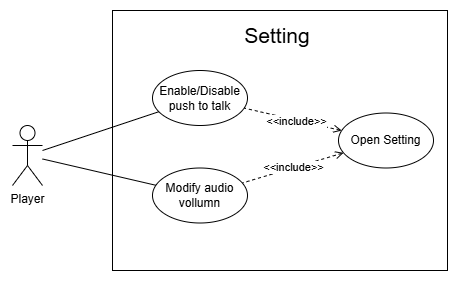
\includegraphics[width=0.75\linewidth]{4.Đặc tả chi tiết các lược đồ/Use-case/images/Setting.png}
    \caption{Use-case mô tả Setting}
    \label{fig:placeholder}
\end{figure}


\begin{table}[H]
\centering
\begin{tabular}{|p{4cm}|p{10cm}|}
\hline
\textbf{Use-case name} & Setting \\ \hline
\textbf{Actor} & Người chơi \\ \hline
\textbf{Descriptions} & Use-case này sẽ chỉ ra các luồng thực thi sau khi mở Setting. \\ \hline
\textbf{Pre-conditions} & Không có \\ \hline
\textbf{Trigger} & Người chơi nhấn nút “SETTINGS” sau khi đã vào lobby hoặc bên ngoài MainMenu. \\ \hline
\textbf{Post-conditions} & Người chơi chọn hành động mà mình muốn thực hiện \\ \hline
\textbf{Normal Flow} &
\begin{enumerate}
\item Nếu đang ở trong lobby thì mở Lobby Menu và nhấn nút "SETTINGS", còn nếu đang ở MainMenu thì chỉ cần nhấn nút "SETTINGS".
\item Người chơi điều chỉnh các thông số.
\item Người chơi nhấn nút "Back" để đóng Setting
\item Use-case kết thúc sau khi Setting được đóng thành công.
\end{enumerate}
\\ \hline
\textbf{Alternative Flow} &
\begin{enumerate}
\item[A1.] Sau khi mở được Setting, nếu người chơi muốn tắt/bật mic của chính mình thì tick vào mục Push-to-talk và nhấn "Save" để lưu.
\item[A2.] Sau khi mở được Setting, nếu người chơi muốn tăng/giảm âm lượng thì kéo slider của mục "Music Volumn" hoặc "Sfx Volumn" tương ứng và nhấn "Save" để lưu.
\end{enumerate}
\\ \hline
\textbf{Exception Flow} &
Không có
\\ \hline
\end{tabular}
\end{table}